%%%%%%%%%%%%%%%%%%%%%%%%%%%%%%%%%%%%%%%%%%%%%%%%%%%%%%%%%%%%%%%%%%%%%%%
% file Starynkevitch-CAIA-RefPerSys-2020mar06.tex
% github.com/bstarynk/web-refpersys
% subdirectory piotr ~/web-refpersys/
% inspired by http://cse.unl.edu/~cbourke/latex/UNLTheme.tex
%%%%%%%%%%%%%%%%%%%%%%%%%%%%%%%%%%%%%%%%%%%%%%%%%%%%%%%%%%%%%%%%%%%%%%%

\documentclass[xcolor=svgnames,final,smaller,a4]{beamer}
\usepackage{relsize}
\usepackage{luacode}
\usepackage{xcolor}
\usepackage{alltt}
\usepackage{wasysym}
\usepackage{verbatim}
\usepackage{hyperref}


\hypersetup{
  colorlinks   = true, %Colours links instead of ugly boxes
  urlcolor     = NavyBlue, %Colour for external hyperlinks
  linkcolor    = DarkGreen, %Colour of internal links
  citecolor   = DarkMagenta, %Colour of citations
  frenchlinks = true,
}
\useoutertheme{split}
\usecolortheme{whale}
\setbeamercolor*{titlelike}{parent=structure}
%\usetheme{AnnArbor}

\title[From CAIA to RefPerSys]{\textsc{From CAIA to RefPerSys} \\
  reflexive, introspective, meta- based AI systems}

\author[B.Starynkevitch \ldots]{Basile \textsc{Starynkevitch} - \href{http://starynkevitch.net/Basile/}{\texttt{starynkevitch.net/Basile}}\\ \href{mailto:basile@starynkevitch.net}{\color{blue}{\texttt{basile@starynkevitch.net}}} - \textsc{92340  Bourg-La-Reine}, France}
  \institute{\textit{RefPerSys} - \href{http://refpersys.org}{\color{red}{\texttt{refpersys.org}}}}

  \date[March 6 \textsuperscript{th}, 2020]{Paris, March 6\textsuperscript{th}, 2020 - seminar in honor of the late J.Pitrat}

 \begin{luacode*}
   local gitpip=io.popen("git log --no-color --format=oneline -1 --abbrev=16 --abbrev-commit -q | cut -d' ' -f1")
   gitid=gitpip:read()
   gitpip:close()
 \end{luacode*}
 \newcommand{\mygitid}{\luadirect{tex.print(gitid)}}
 \newcommand{\RefPerSys}{\href{http://refpersys.org}{\textsc{RefPerSys}}}

 %%%%%%%%%%%%%%%%%%%%%%%%%%%%%%%%%%%%%%%%%%%%%%%%%%%%%%%%%%%%%%%%
  \begin{document}

 \begin{frame}
   \begin{relsize}{-0.5}
     \titlepage
     
     {\textcolor{brown}{{\large \textbf{Opinions are only mine}}}} \hspace{0.5cm}{\relsize{-1}{git commit \texttt{\mygitid}}}

   \begin{relsize}{-0.5}
       {these slides are under} \raisebox{-0.2cm}{
\includegraphics[width=0.12\textwidth]{CC-BY-SA-4}} \href{https://creativecommons.org/licenses/by-sa/4.0/}{Creative Commons Attribution-ShareAlike 4.0 International}
        
        My employer {\relsize{-0.5}{(or funding agencies at work)}} would probably
        disagree with most of my opinions here. Any agreement with my employer's
        policies or positions is accidental.
        
   \end{relsize}
   
   \end{relsize}
 \end{frame}

\begin{frame}{Overview}
\tableofcontents
\end{frame}

 \section{What is AI?}
 \label{sec:what-is-ai}
 
 \begin{frame}
   \frametitle{What is AI?}
   \begin{itemize}
   \item \textcolor{red}{\large \textbf{A}}rtificial
     \textcolor{red}{\large \textbf{I}}ntelligence (and
     \href{https://en.wikipedia.org/wiki/AI_winter}{AI winter} - predicted by J.Pitrat)
     \begin{itemize}
       \item \textbf{A}rtificial \textbf{G}eneral \textbf{I}ntelligence 
       \item symbolic \textbf{A}rtificial \textbf{I}ntelligence
       \item machine learning  \textbf{A}rtificial \textbf{I}ntelligence
       \item\textbf{A}rtificial \textbf{I}ntelligence applications
     \end{itemize}
   \item \textcolor{red}{\large \textbf{A}}dvanced  \textcolor{red}{\large \textbf{I}}nformatics
   \item \textbf{A}bstract \textbf{I}nterpretation {\relsize{-1}{(a
       technique for static program analysis, by
       Cousot)}}\\
     $\rightarrow$ IMHO it could be the next ``AI winter''\\
     \relsize{-1}{I am impatiently waiting for
       \href{http://frama-c.com/}{Frama-C} fully automated analysis of
       \href{https://www.tensorflow.org/}{\textsc{TensorFlow}} C++
       code (its \href{https://floating-point-gui.de/}{floating point} precision issues), or of
       \href{https://github.com/bstarynk/caia-pitrat/}{\textsc{Caia}}
       C code {\large \smiley{}}; the ``\textcolor{brown}{robust AI}'' buzzword....}
   \end{itemize}


   \bigskip

   \begin{block}{philosophical question}
     Is AI a science unrelated to computer science, or is it part of it?
   \end{block}

   \begin{relsize}{-1.5}
     (probable major disagreement between J.Pitrat and me)
   \end{relsize}
   
 \end{frame}
     
 \begin{frame}
   \frametitle{Why AI systems are needed? hard problems (1/2)}

   Because mankind or nations or continents -and decision makers-
   face major problems which are not fully understood (incomplete list) :

   \begin{itemize}
   \item \href{https://en.wikipedia.org/wiki/Global\_warming}{global
     warming},
     \href{https://en.wikipedia.org/wiki/Malnutrition}{malnutrition}
     and \href{https://en.wikipedia.org/wiki/Pollution}{pollution}
   \item the [co-] design and operation of complex systems (nuclear
     power plants -\href{https://en.wikipedia.org/wiki/ITER}{ITER}-,
     autonomous transportation,
     \href{https://en.wikipedia.org/wiki/Smart_grid}{smart grids}, \href{https://en.wikipedia.org/wiki/Super_grid}{super grid},
     \href{https://en.wikipedia.org/wiki/Smart_city}{smart cities},
     communication networks,
     \href{https://en.wikipedia.org/wiki/Water\_distribution\_system}{water
       distribution system},
     \href{https://en.wikipedia.org/wiki/Cobot}{cobots})
   \item managing complex systems (e.g. the
     \href{https://en.wikipedia.org/wiki/World\_Wide\_Web}{World Wide
       Web}) or their implementation (fiber optics deployment in
     France) or organizations
     (\href{https://www.velib-metropole.fr/}{Vélib}) - avoiding \href{https://en.wikipedia.org/wiki/Boreout}{boreout}
     \item \href{https://en.wikipedia.org/wiki/Digital_twin}{digital
       twins} (e.g. of an automobile, of holiday travels) and
       distributed
       \href{https://en.wikipedia.org/wiki/Embedded_system}{embedded
         systems} (or
       \href{https://en.wikipedia.org/wiki/Edge_computing}{edge
         computing})
     \item macro-economical policies of the Euro zone (why negative interest rates?)
     \item fighting global bio-viruses (e.g. coronavirus = closed
       software + chemistry)
   \item in France: retirement policies (why is it difficult to simulate?)
   \end{itemize}

 \end{frame}

 
 \begin{frame}
   \frametitle{Why AI systems are needed? hard problems (2/2)}

   \begin{itemize}
   \item in general: defining useful regulations (e.g. $CO_2$ global
     market, world-wide distribution of economical wealth,
     \href{https://en.wikipedia.org/wiki/Neuroeconomics}{neuroeconomics})
   \item political problems: peace in Middle East?
   \item lack of motivated software developers (how to keep their
     motivations and productivity?) - see \href{https://en.wikipedia.org/wiki/Bullshit_Jobs}{\textit{Bullshit jobs}} and \href{https://www.editions-observatoire.com/content/La_comédie_inhumaine}{\textit{La comédie (in)humaine}}
   \item going to Mars, \href{https://en.wikipedia.org/wiki/Terraforming\_of\_Mars}{terraforming it}, \href{https://en.wikipedia.org/wiki/Colonization_of_Mars}{colonizing it}
   \item understanding the physical world (particle physics, quantum
     physics, exobiology, cosmology?) and improving it
     (\href{https://en.wikipedia.org/wiki/Climate-smart_agriculture}{climate-smart
       agriculture}, world-wide better
     \href{https://en.wikipedia.org/wiki/Energy\_mix}{energy mix})
   \item understanding and repairing the human body (whole body
     digital twin? neurology?
     \href{https://en.wikipedia.org/wiki/Oncology}{oncology}?
     \href{https://en.wikipedia.org/wiki/Neurosurgery}{neurosurgery}, \href{https://en.wikipedia.org/wiki/Obesity}{obesity})
     \item understanding and improving the Internet (it could be very
       brittle?)
     \item understanding and improving the French law (online, but how much is it consistent?)
     \item improving communication and trust between human beings
   \end{itemize}

 \end{frame}
 
 \begin{frame}
   \frametitle{Why AI systems need to be free software? (1/2)}

   The \href{https://www.gnu.org/philosophy/free-sw.en.htm}{\textsc{Gnu FSF}} defines free software :
   \begin{itemize}

    \item The freedom to run the program as you wish, for any purpose (freedom 0).
    \item The freedom to study how the program works, and change it so it does your computing as you wish (freedom 1). Access to the source code is a precondition for this.
    \item The freedom to redistribute copies so you can help others (freedom 2).
    \item The freedom to distribute copies of your modified versions to others (freedom 3). By doing this you can give the whole community a chance to benefit from your changes. Access to the source code is a precondition for this.

   \end{itemize}

   ``\textcolor{red}{\textbf{What is free software and why it is important to \emph{society}}}''

   \medskip
   
 The ``source code''
 \href{https://en.wikisource.org/wiki/The_Open_Source_Definition}{being
   defined} as : ``The source code must be the preferred form in which
 a programmer would modify the program''
 \end{frame}

 \begin{frame}
   \frametitle{Why AI systems need to be free software? (2/2)}

   See also \href{https://laboutique.edpsciences.fr/produit/1107/9782759824304/Le\%20fabuleux\%20chantier}{
   Le fabuleux chantier : Rendre l’intelligence artificielle
   robustement bénéfique {\relsize{-1.5}{(The fabulous project: making
       artificial intelligence robustly beneficial)}}}

   Notice analogy between free software / open source and academical [mis-]practices

   \bigskip
   

   \begin{itemize}
   \item
     \href{https://en.wikipedia.org/wiki/Publish_or_perish}{publish or
       perish}. Pitrat observed that there is not enough incentive to
     make real-sized AI \emph{software systems} (not toy demos) and
     favoring experimental approaches.

   \item \href{https://www.nber.org/papers/w7600}{\textit{The Simple Economics of Open Source}}

   \item \href{https://cryptome.org/2015/07/big-other.pdf}{\textit{Big other: surveillance capitalism and the prospects of an information civilization}}
   \end{itemize}

   \medskip
   
   See \href{https://softwareheritage.org/}{\texttt{softwareheritage.org}}
   and dream of mega  knowledge bases
 \end{frame}

 \begin{frame}
   \frametitle{Pitrat's thesis}
   \begin{block}{about intelligence}
     \textbf{There is no \emph{\textcolor{brown}{simple} theory} or \emph{\textcolor{brown}{simple} model} of intelligence} (be it artificial or natural).\\
     $\Rightarrow$ any AI system has to be complex (with chaotic behavior) and evolving!     
 \end{block}

 Pitrat's analogy: a bird can fly, an airplane also fly, they are
 designed differently.


 \begin{itemize}
 \item \textbf{\textcolor{red}{experimentation is king}}

 \item \textbf{\textcolor{red}{theoretical limitations}} (affecting humans too!) \textcolor{red}{do
   not matter \textbf{in practice} :}
   \begin{enumerate}
   \item \href{https://en.wikipedia.org/wiki/Halting_problem}{halting problem}
   \item \href{https://en.wikipedia.org/wiki/Rice\%27s_theorem}{Rice's theorem}
   \item \href{https://en.wikipedia.org/wiki/Gödel's_incompleteness_theorems}{Gödel's incompleteness theorems}

   \item \href{https://en.wikipedia.org/wiki/Church–Turing_thesis}{Church-Turing thesis}

   \item \href{https://en.wikipedia.org/wiki/Curry–Howard_correspondence}{Curry–Howard correspondence}; \\
     see {\href{https://xavierleroy.org/}{\textit{Software, between mind and matter}}} (X.Leroy)

   \item heuristically and \textbf{\textcolor{DarkGreen}{usually}} avoiding \href{https://en.wikipedia.org/wiki/Combinatorial_explosion}{combinatorial explosion}
     
   \end{enumerate}
   
 \end{itemize}
 \end{frame}

 \begin{frame}
   \frametitle{consequences of Pitrat's thesis}

   \begin{relsize}{+1}
 \textcolor{brown}{\textbf{AI systems have to be \emph{globally}
     inconsistent}} (like humans are) and \href{https://en.wikipedia.org/wiki/Antifragile}{\textbf{\emph{antifragile}}} (Taleb)
   \end{relsize}

   \begin{itemize}
     \item importance of ``insight'' :
       \href{https://en.wikipedia.org/wiki/Eureka\_effect}{Eureka
         effect} (``Aha! moment'')
     \item intelligent systems cannot be fully modular or
       compositional to have an
       \href{https://en.wikipedia.org/wiki/Emergence}{emerging}
       intelligent behavior with
       \href{https://en.wikipedia.org/wiki/Self-organization}{self-organization}
       \item theoretical quasi-impossibility to explain or modelize
         intelligence.
       \item AI systems are non-modular and will exhibit
         non-reproducible behavior \\ $\Rightarrow$
         \href{https://en.wikipedia.org/wiki/Randomized_algorithm}{randomized
           algorithms} are practically essential to AI!
       \item \textcolor{brown}{\textbf{time is important in AI systems}} (see 
         \href{http://man7.org/linux/man-pages/man7/time.7.html}{\texttt{time(7)}} on Linux)

         \item importance of
           \href{https://en.wikipedia.org/wiki/Self-awareness}{self-awareness}
           and
           \href{https://en.wikipedia.org/wiki/Introspection}{introspection}
           for intelligent systems (on Linux could be done with
           \href{https://github.com/ianlancetaylor/libbacktrace}{\texttt{libbacktrace}},
           conceptually related to
           \href{https://dl.acm.org/doi/10.1007/BF01019459}{the
             discoveries of continuations})
   \end{itemize}

   Since AI systems need to have some kind of randomness (see
   \href{http://man7.org/linux/man-pages/man4/random.4.html}{\texttt{random(4)}} on Linux),
   \textcolor{red}{\textbf{experimental reproducibility is \emph{ethically} important}}.
 \end{frame}


 \section{Engineering aspects of AI software systems}
 \label{sec:engineering-ai}
 
 \begin{frame}
   \frametitle{Engineering aspects of software (1/2)}

   We need a computer to run a software:

   \begin{center}
     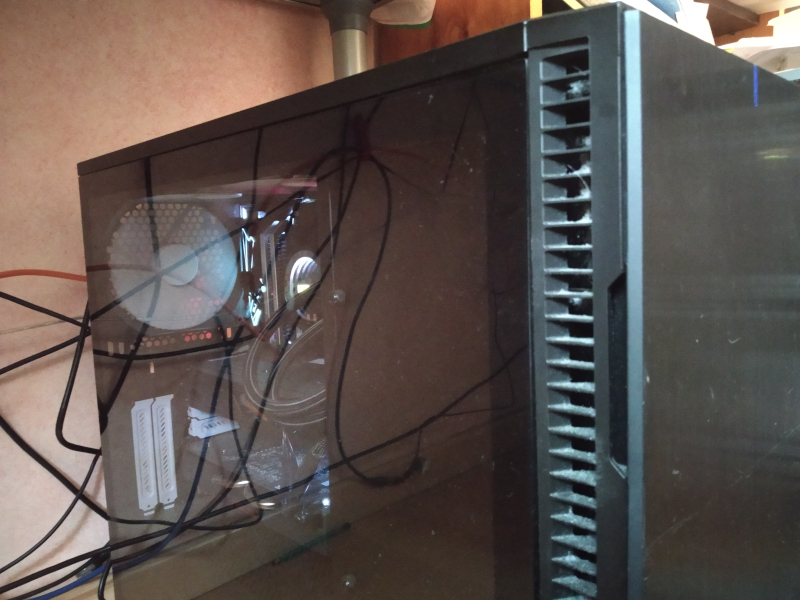
\includegraphics[width=0.55\textwidth]{black-box-computer-small}\\
     (photo by \href{http://matthieu-starynkevitch.com/}{Matthieu Starynkevitch})
   \end{center}

   \relsize{-0.5}{(we look inside the box and see things -cables- which are \emph{not} inside but reflected)}
 \end{frame}

 \begin{frame}
   \frametitle{Engineering aspects of software (2/2)}
 
   But J.Pitrat wrote (in \href{https://onlinelibrary.wiley.com/doi/book/10.1002/9780470611791}{\textit{Artificial Beings}}, §4 p67):
   
   \begin{relsize}{+1}
   \begin{quote}
     The black box is the opposite of consciousness, and we must \textcolor{brown}{always} avoid it
   \end{quote}
   \end{relsize}
   
   and later (\textit{Artificial Beings} p259):

   \begin{relsize}{+1}
   \begin{quote}
       \textsc{Caia} uses \textcolor{brown}{two} programs that it has not written: \href{http://gcc.gnu.org/}{\textsc{Gcc}} and \href{https://https://en.wikipedia.org/wiki/Linux}{\textsc{Linux}}
     \end{quote}
   \end{relsize}
   
   {\relsize{-2}{emphasis is mine; I will dare doing some nitpicking}}

   \bigskip
   
   My black box runs \textsc{Caia} {\large \smiley{}}
 \end{frame}


 \begin{frame}
   \frametitle{D.Wheeler's \texttt{sloccount}}

 A \textbf{machine learning} approach to \textbf{\textcolor{red}{estimate software development costs}} by
 counting source lines of code (SLOC), and free (GPL) software
 measuring that, on
 \href{https://dwheeler.com/sloccount/}{\textbf{\texttt{dwheeler.com/sloccount/}}}.

 A good programmer is rumored to be able to write about 30K SLOC per
 year and this depends not much on the programming language used by
 him (if he is expert on that language).
 \medskip
 

 Some figures (from \href{https://en.wikipedia.org/wiki/Source_lines_of_code}{Source lines of code} wikipage) :
 \begin{tabular}{lcp{0.4\textwidth}}
   \textbf{software} & \textbf{source size} & \\
   Debian 7 & 419 MSLOC & the old Debian 7 distribution \\
   Linux 3.6 & 15.9 MSLOC & the Linux 3.6 kernel \\
 \end{tabular}

 \bigskip
 
\href{https://en.wikipedia.org/wiki/Software_development_effort_estimation}{Estimating
  software development costs} is tricky: half of software projects are
``failing''; refactoring a code base may involve replacing ten
thousands lines by just one thousand of better lines.

\medskip

But software code size remains a good measure for its development
costs.
 \end{frame}


 \begin{frame}
   \frametitle{source code measurement of \textsc{Caia}}

   From \href{https://github.com/bstarynk/caia-pitrat}{\texttt{github.com/bstarynk/caia-pitrat}}, the C lines being generated :

   \begin{relsize}{-1}
   \begin{alltt}
  SLOC	Directory	SLOC-by-Language (Sorted)\\
506558  caia-pitrat     ansic=506160,sh=281,perl=63,cpp=54\\

Totals grouped by language (dominant language first):\\
ansic:       506160 (99.92\%)\\
sh:             281 (0.06\%)\\
perl:            63 (0.01\%)\\
cpp:             54 (0.01\%)\\

Total Physical \textcolor{Navy}{\textbf{Source Lines of Code}} (SLOC)                = \textcolor{red}{\textbf{\large 506,558}}\\
Development Effort Estimate, \textcolor{Navy}{\textbf{Person-Years}} (Person-Months) = \textcolor{red}{138.32} (1,659.86)\\
 (Basic COCOMO model, Person-Months = 2.4 * (KSLOC**1.05))\\
Schedule Estimate, Years (Months)                         = 3.49 (41.84)\\
 (Basic COCOMO model, Months = 2.5 * (person-months**0.38))\\
Estimated Average Number of Developers (Effort/Schedule)  = 39.67\\
\textcolor{Navy}{\textbf{Total Estimated Cost to Develop}}                           = {\relsize{+1}{\textcolor{red}{\$ 18,685,394}}}\\
 (average salary = \$56,286/year, overhead = 2.40).\\
SLOCCount, Copyright (C) 2001-2004 David A. Wheeler
   \end{alltt}
   \end{relsize}
 \end{frame}
 
 \begin{frame}
   \frametitle{other source code measures}

 \begin{tabular}{lcp{0.55\textwidth}}
   \textbf{software} & \textbf{source size} & \\
   CAIA & 506KLOC & \textsc{Caia} as before \\
   Linux 3.6 & 15.9 MSLOC & the Linux 3.6 kernel on \href{https://kernel.org/}{\texttt{kernel.org}} \\
   Xorg 1.12 & 406KLOC & The X11 window display server on \href{https://www.x.org/}{\texttt{www.x.org}}  \\
   GCC 9.2 & 5.605MLOC & The GCC compiler on \href{https://gcc.gnu.org/}{\texttt{gcc.gnu.org}} \\
   binutils 2.34 & 2.104MLOC & GNU assembler and linker \href{https://www.gnu.org/software/binutils/}{\texttt{www.gnu.org/software/binutils/}} \\
   bash 5.0 & 124KLOC & GNU Bourne Again SHell \href{https://www.gnu.org/software/bash/}{\texttt{www.gnu.org/software/bash/}} \\
   glibc 2.31 & 1.257MLOC & GNU C library \href{https://www.gnu.org/software/libc/}{\texttt{www.gnu.org/software/libc/}} \\
   libbacktrace & 18.9KLOC & backtracking {\relsize{-1.5}{\href{https://github.com/ianlancetaylor/libbacktrace}{\texttt{github.com/ianlancetaylor/libbacktrace}}}} \\
   Qt5 & 23.799MLOC & a C++ GUI toolkit \href{https://qt.io/}{\texttt{qt.io}}\\
   GNU readline & 36.6KLOC & a line editor library \href{https://www.gnu.org/software/readline/}{\texttt{www.gnu.org/software/readline/}} \\
 \end{tabular}
 
 \end{frame}
 \begin{frame}
   \frametitle{illusion about C compiler}

   J.Pitrat told me:
   \begin{quote}
     Only a small amount of the C language is used by \textsc{Caia} so I don't depend that much on GCC
   \end{quote}

   But \href{https://gcc.gnu.org/onlinedocs/gcc/Invoking-GCC.html}{using} \texttt{gcc -O2 -ftime-report} shows that about 80\% of GCC optimization passes are used.

   \bigskip
   
   See some pages of
   \href{http://starynkevitch.net/Basile/bismon-chariot-doc.pdf}{my
     Bismon draft report} for an explanation.

   GCC optimizations are surprising.

   \bigskip

   Disabling optimizations would lower \textsc{Caia} performance by
   perhaps 30\%. See also
   \href{https://en.wikipedia.org/wiki/Tiny_C_Compiler}{TinyCC}.
 \end{frame}

 \begin{frame}
   \frametitle{The Joel Test: 12 Steps to Better Code}
   From \href{https://dev.to/checkgit/the-joel-test-20-years-later-1kjk}{\texttt{dev.to/checkgit/the-joel-test-20-years-later-1kjk}}
   \begin{relsize}{-1.0}
     \begin{enumerate}
       \item Do you use \href{http://git-scm.com/}{Git}, or some lesser source control system?
       \item Can you build and release in one step?
       \item Do you build and test before merging to master? \textcolor{red}{\texttt{\relsize{+1}{make bootstrap}}} in \href{https://gcc.gnu.org/}{\textit{GCC}}
    \item Do you have a bug database?
    \item Do you fix bugs before writing new code?
    \item Do you have an up-to-date schedule?
    \item Do you write a spec before writing code?
    \item Do programmers have quiet working conditions free of interruptions?
    \item Do you use the best development tools money can buy?
    \item Do you have human testers?
    \item Do you have automated testing?
     \end{enumerate}
   \end{relsize}
   with \href{https://en.wikipedia.org/wiki/Code_review}{code reviews}
   (e.g. \href{https://gcc.gnu.org/ml/gcc-patches/}{\texttt{gcc-patches@gcc.gnu.org}})
 \end{frame}

 \begin{frame}
   \frametitle{The Magical Number $7 \pm 2$ }

   \begin{block}{\href{https://en.wikipedia.org/wiki/The_Magical_Number_Seven,_Plus_or_Minus_Two}{Miller's law} (1956)}
     the number of objects an average person can hold in working
     memory is about seven
   \end{block}

   \bigskip
   
   This empirically holds for software developers, computer scientists
   and human artificial intelligence researchers.

   \medskip
   
   $\rightarrow$ a software whose
   \href{https://en.wikipedia.org/wiki/Cyclomatic_complexity}{cyclomatic
     complexity} (Mc.Cabe 1976) is above 7 will probably remain
   undebuggable, and complex software are always buggy.

   \medskip
   
   $\rightarrow$ avoid spaghetti code in human written programs. But that does not matter for machine generated code.

 \end{frame}

 \begin{frame}
   \frametitle{Miller's law in AI}
   
   
   $\rightarrow$ the types of functions in human written functional
   style programs remains reasonable. Pathological cases of
   \href{https://en.wikipedia.org/wiki/Type_inference}{type inference}
   are practically rare.

   \medskip
   So \href{https://en.wikipedia.org/wiki/Modular_programming}{modular
     programming}\footnote{Generated code could be non-modular!} or
   \href{https://en.wikipedia.org/wiki/Object-oriented_programming}{object-oriented
     programming} is for humans. Hence
   \href{https://en.wikipedia.org/wiki/Just-in-time_compilation}{Just-in-time
     compilation} techniques (e.g. devirtualization of
   \href{https://en.wikipedia.org/wiki/Virtual_method_table}{virtual
     method tables}) are practically efficient.


   \medskip

   Few functions get much more than 6 or 7 arguments


   \begin{block}{Miller's law in AI system}
   Is there one? Do AI systems have a short memory threshold?

   Is the 7 threshold related to mathematical properties of semantic networks (diameter of reference graphs)
   \end{block}
   
 \end{frame}

\begin{frame}
 \frametitle{What should really matter in an AI system}

 \begin{itemize}
   
 \item \textcolor{red}{\textbf{explicit some
     \href{https://en.wikipedia.org/wiki/Trusted_computing_base}{trusted
       computer base}}}, that is all the things

   \begin{itemize}
   \item hardware components (motherboard, keyboard, mouse, screen, Ethernet)
   \item low-level software components (firmware: BIOS, UEFI, graphics card firmware)
   \item operating system kernel (Linux kernel)
   \item middleware software components (compiler, user interface,
     operating system, file systems, databases)
   \end{itemize}
   
   the AI system depends on. Getting rid of every software component
   is practically futile {\relsize{-1}{(billions of source lines in a Linux desktop ; see
   also
   \href{http://linuxfromscratch.org/}{\texttt{\textcolor{Sienna}{linuxfromscratch.org}}}
   which is bootstrapped)}}.

   \item \textcolor{red}{\textbf{take advantage of most
       \emph{existing} computing resources}} (multi-core, cache
     locality, disk, MMU, Internet) \textcolor{red}{\textbf{and
         \emph{existing} software components}}.

   \item \textcolor{red}{\textbf{give \emph{declarative} knowledge
       to your AI system about efficiently using \emph{existing}
       open source software components}} which are choosen by humans
     
   \end{itemize}

 \end{frame}

 \begin{frame}
   \frametitle{AI software and computers ``are'' semantics networks}
 

 From wikipedia
 \href{https://en.wikipedia.org/wiki/Semantic_network}{Semantic
   network} {\relsize{-1}{(but imagine hundred of thousands of nodes and labelled arrows)}}

 \bigskip

 \begin{center}
 
\includegraphics[width=0.55\textwidth]{Semantic-Net}
 \end{center}
 
 \bigskip
 
 $\Rightarrow$ Flexible frame representation, including knowledge
 representation of various ``expertises'' about how to use existing
 ``trusted'' software components (cf
 \href{https://www.decoder-project.eu/}{\textsc{Decoder}} project) and
 how to generate code.
 \end{frame}

 \begin{frame}
   \frametitle{Brook's law}

   From \href{https://en.wikipedia.org/wiki/The_Mythical_Man-Month}{\textit{The Mythical Man-Month}} (F.Brooks, 1975):

   Its central theme is that "adding manpower to a late software project makes it later".
   
   {\relsize{-1}{while it takes one woman nine months to make one baby, "nine women can't make a baby in one month"}

   it takes some incompressible time to make a bootstrapped AI system.}
   

   \medskip

   and there is \href{https://en.wikipedia.org/wiki/No_Silver_Bullet}{\textit{No silver bullet}}

   \smallskip
   
   \hrule

   \medskip
   
   Communication between software developers (or between artificial intelligence researchers) matters.
   \emph{Open source} software is an effective communication channel.

   \medskip

   \href{https://en.wikipedia.org/wiki/Heisenbug}{Heisenbugs} and
   heisenmetabugs.  Also
   \href{https://en.wikipedia.org/wiki/Cargo_cult_programming}{Cargo
     cult programming} and
   \href{https://en.wikipedia.org/wiki/Rubber_duck_debugging}{rubber
     duck debugging} (and usefulness of code reviews, even by junior programmers)
   
 \end{frame}

 \begin{frame}
   \frametitle{Hofstater's law}

   \begin{block}{\href{https://en.wikipedia.org/wiki/Hofstadter's_law}{Hofstadter's law}}
     It always takes longer than you expect, even when you take into account Hofstadter's Law.
   \end{block}

   Very true of development of AI systems (or of preparing slides like
   these ones). See
   \href{https://en.wikipedia.org/wiki/Gödel,_Escher,_Bach}{\textit{Gödel,
       Escher, Bach: An Eternal Golden Braid}}

   \bigskip

   Related:
   \href{https://en.wikipedia.org/wiki/I_Am_a_Strange_Loop}{\textit{I
       am a strange loop}} and
   \href{https://en.wikipedia.org/wiki/Ship_of_Theseus}{Ship of
     Theseus paradox} (relevant to bootstrapped AI systems)
   
 \end{frame}

 \begin{frame}
   \frametitle{the staircase development model of bootstrapped AI}

   Illustrated with \RefPerSys, applicable to CAIA:

   \begin{center}
     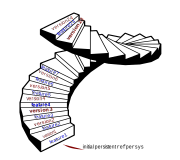
\includegraphics[width=0.4\textwidth]{spiral-stairs}
   \end{center}

   \smallskip
   

  \begin{quote}
    \begin{relsize}{-0.5}
    Each new feature -or small incremental change or a few of them
    (small \texttt{git commit}s) - of {\RefPerSys} enables us to build
    and \textbf{generate} the next version of {\RefPerSys}, and a next
    feature is then added to that \textit{improved} version, and so on
    repeatedly, etc....
    \end{relsize}
  \end{quote}
   
 \end{frame}
 
 %================================================================

 \section{CAIA in practice}

 \begin{frame}
   \frametitle{CAIA demo}

   \texttt{git clone
     \href{https://github.com/bstarynk/caia-pitrat.git}{https://github.com/bstarynk/caia-pitrat.git}}. You
   need 250Mbytes of disk space.

   \texttt{cd caia-su-24feb2016}
   
Observe the buggy generated \texttt{dx.h} 

   \texttt{make} perhaps needed twice (15 minutes of CPU time).

   \texttt{./caia}

   Observe the \texttt{ed} like user interface. Try \texttt{L EDITE} perhaps twice.
    
   Look into \texttt{\_*} persistent data files. Too small to be
   friendly with most file systems. See figure on
   \href{https://en.wikipedia.org/wiki/Ext2}{Ext2} wikipage. Read
   about \href{https://en.wikipedia.org/wiki/File_system}{file
     systems} some
   \href{http://pages.cs.wisc.edu/~remzi/OSTEP/}{Operating Systems
     textbook}.

   Use
   \href{http://man7.org/linux/man-pages/man1/strace.1.html}{strace(1)}
   to find out that the date is displayed by running the \texttt{date}
   command. But see
   \href{http://man7.org/linux/man-pages/man7/time.7.html}{time(7)}

   No
   \href{https://en.wikipedia.org/wiki/C_dynamic_memory_allocation}{C
     dynamic memory allocation} using
   \href{http://man7.org/linux/man-pages/man3/malloc.3.html}{malloc(3)}. That
   was a design mistake.
   
 \end{frame}
 
 \begin{frame}
   \frametitle{some software I wrote for J.Pitrat}
m
   \begin{itemize}
     \item \texttt{manydl.c} under \texttt{git clone
       \href{https://github.com/bstarynk/misc-basile.git}{https://github.com/bstarynk/misc-basile.git}}
       generates random C code, compiles each of them as a
       plugin. Shows that a Linux program can
       \href{http://man7.org/linux/man-pages/man3/dlopen.3.html}{dlopen(3)}
       ``simultaneously'' many hundreds of thousands of plugins.

    \item\texttt{git clone
      \href{https://github.com/bstarynk/minil.git}{https://github.com/bstarynsk/minil.git}}
      deals with dynamically allocated frames (persisted in
      \href{http://json.org}{JSON} format with
      \href{http://www.digip.org/jansson/}{\texttt{libjansson}}) and
      \texttt{readline} command line interface with
      auto-completion. French comments, GPLv3+ (could be used by some
      intern as a starting point).
      
   \end{itemize}
 \end{frame}

   %%%%%%%%%%%%%%%%%%%%%%%%%%%%%%%%%%%%%%%%%%%%%%%%%%%%%%%%%%%%%%%%

   \section{RefPerSys - a future successor to CAIA}
   \label{sec:refpersys}

  \begin{frame}
     \frametitle{{\RefPerSys} - early work in progress}

     A future successor to CAIA for Linux/x86-64 (GPLv3+, open science). A
     bootstrapped AI system. An acronym for \textbf{Ref}lexive
     \textbf{Per}sistent \textbf{Sys}tem. See
     \href{http://refpersys.org/}{\large\texttt{\textbf{\textcolor{red}{refpersys.org}}}}
     and code (C++ and persistent JSON data) on
     \href{https://gitlab.com/bstarynk/refpersys/}{\texttt{\textbf{https://gitlab.com/bstarynk/refpersys/}}}

     \begin{center}
       \includegraphics[width=0.60\textwidth]{refpersys-logo} \\
       \relsize{-2}{SVG logo by Gaëtan Tapon (Paris, France)}
     \end{center}
     
     With contributions from Abhishek Chakravarti and Nimesh Neema (India). Active additional contributors welcome.

     Coded in C++ (some of which is generated). For Qt graphical interface.
  \end{frame}

  \begin{frame}
    \frametitle{immutable values of \RefPerSys}

    Each value has a class. ObjVLisp model. Most values are immutable, except objects. They are dynamically allocated and garbage collected

    \begin{itemize}
    \item tagged 63 bits integers
    \item boxed doubles
    \item boxed UTF-8 strings
    \item mutable objects
    \item ascending sets of objects
    \item tuples of objects
    \item closures (the closed ``variables'' are values, the connective gives the function)
    \item immutable instances with components (values)
    \item boxed Qt pointers (to widgets)
      \item boxed JSON
      \item etc \ldots
    \end{itemize}
    
  \end{frame}
  
 

  \begin{frame}
    \frametitle{mutable objects of \RefPerSys}
s
    Each object has :
    \begin{itemize}
    \item a fixed random ``globally'' unique object id (96 bits) externally represented by a oid string like \texttt{\_02iWbXmFx8f04ldLRt}. So objects are comparable by their oid.
    \item a mutex for multi-thread locking
      \item a modification time (double)
      \item a mutable class (itself an object reference)
      \item a space (itself an object reference, or nil) for persistence
    \item a finite mapping (varying with time) for attribute entries. Each entry has a key which is an object, associated to a non-nil value. Every key is different.
    \item a varying vector for object components
    \item an optional mutable payload
      \item two atomic C++ function pointers (one for magic attribute getting, another for applying closures having that object as connective).
    \end{itemize}
    
  \end{frame}
  
  \begin{frame}
    \frametitle{mutable payload in objects of \RefPerSys}

    They hold any additional data not fitting elsewhere:
    \begin{itemize}
    \item class information (method dictionnary + superclass)
    \item symbol information
    \item string buffers
    \item mutable vectors of doubles
    \item mutable vectors of values
    \item mutable sets (e.g. \texttt{std::set})
    \item mutable relations
    \item dictionnaries associating strings to values or object
    \item Qt windows
    \item file or process or database handles
    \item etc...
    \end{itemize}

    Objects and their payload may represent a semantics network
  \end{frame}
   
  \begin{frame}
    \frametitle{persistence in \RefPerSys}
    The entire heap is dumped before exit and reloaded just after startup. Using JSON (so in a textual format friendly to \texttt{git}).

    \begin{itemize}
    \item some values are transient (Qt widgets, transient closures or instances).
    \item most values are persistent.
    \item objects are shared and persistent in their space.
    \item continuations (call stack) are not persisted; using \texttt{libbacktrace}
    \end{itemize}
  \end{frame}

  \begin{frame}
    \frametitle{graphical user interface in \RefPerSys}
    \begin{itemize}
    \item several Qt windows
    \item auto-completion
    \item syntax oriented editor (Centaur inspired)
    \item model view controller approach above flexible \RefPerSys object model
    \end{itemize}
  \end{frame}
  
  \begin{frame}
    \frametitle{agenda machinery in \RefPerSys}

    To be implemented:
    
    \begin{itemize}
    \item multi-threaded, multi-workers (e.g. a dozen of worker threads)
    \item several queues of tasklets
    \item each tasket is an object, conceptually a sort of bytecode VM
    \item each worker thread runs a tasklet for a few milliseconds. That run could modify the agenda by adding/removing/reorganizing tasklets in it
    \item the Qt GUI may add tasklets to the agenda
      \item the agenda should be partly persistent
    \end{itemize}
  \end{frame}

  \begin{frame}
    \frametitle{future work}
    \begin{itemize}
    \item generating most of C++ code (Quine), including persistence, Qt, GC
    \item perhaps interfacing \texttt{libgccjit}  -runtime generation of code
    \item rule based approach
    \item metarules compiled to code
    \item richer frame model
    \item climbing the staircase with higher-level (more declarative) representations
    \item declarative knowledge to use machine learning libraries
        \href{https://www.tensorflow.org/}{\textit{TensorFlow}},
        \href{http://gudhi.gforge.inria.fr/}{\textit{Ghudi}}
      \item self-tuning approach à la
        \href{https://en.wikipedia.org/wiki/MILEPOST\_GCC}{MILEPOST
          GCC}
      \item declarative knowledge about other major C++ open source libraries and generate C++ code calling them.
    \end{itemize}
  \end{frame}
 
  \begin{frame}
    \frametitle{why generate C++? ~ (1/2)}

    Mostly for social reasons: C++11 or C++17 is well known, with robust compilers. Also
    \begin{itemize}
    \item C++11 has powerful \href{https://en.cppreference.com/w/cpp/container}{standard containers}
    \item C++ is compatible with C, and \texttt{dlopen}-able on
      Linux: \href{https://www.tldp.org/HOWTO/html_single/C++-dlopen/}{C++
        dlopen mini HowTo}
      \item I worked inside \href{http://gcc.gnu.org/}{GCC}, which
        accepts
        \href{https://gcc.gnu.org/onlinedocs/gccint/Plugins.html}{plugins}
        coded in C++.
      \item C++ is multi-threaded
      \item C++17 don't have
        \href{https://en.wikipedia.org/wiki/Flexible_array_member}{flexible
          array members} yet but in practice on Linux/x86-64 we can use
        with care (as in C89) last fields which are arrays of dimension
        0.
      \item C++ has \href{https://en.cppreference.com/w/cpp/language/lambda}{closures} and smart pointers.
    \end{itemize}

  \end{frame}

  
  \begin{frame}
    \frametitle{why generate C++? ~ (2/2)}

    Also
    \begin{itemize}

      \item existing C++ compilers optimize very well (but slowly).
      \item C++ on Linux is compatible with
        \href{https://gcc.gnu.org/onlinedocs/jit/}{libgccjit} and/or
        \href{https://asmjit.com/}{asmjit} for just-in-time
        generation of code at runtime.
      \item many reputable interesting C++ (or C) libraries exist
        (\href{https://github.com/open-source-parsers/jsoncpp}{JsonCpp},
        \href{https://tensorflow.org/}{TensorFlow},
        \href{https://project.inria.fr/gudhi/}{Ghudi},
        \href{https://qt.io/}{Qt},
        \href{https://pocoproject.org/}{POCO},
        \href{https://gmplib.org/}{GMPlib} etc....)
    \end{itemize}

    \bigskip
    
   But C++ is an ugly monster
   (\href{http://www.open-std.org/jtc1/sc22/wg21/docs/papers/2012/n3337.pdf}{n3337}
   has 1324 pages) which I don't know and it is compiled slowly. Be aware
   and scared of
   \href{http://blog.llvm.org/2011/05/what-every-c-programmer-should-know.html}{undefined
     behavior}.

   \medskip
   
    Other language implementations could have been considered:
    \href{http://rust-lang.org/}{Rust},
    \href{https://go-lang.org/}{Go}, \href{https://sbcl.org/}{SBCL},
    \href{https://www-sop.inria.fr/mimosa/fp/Bigloo/}{Bigloo},
    \href{https://ocaml.org/}{Ocaml},
    \href{http://www.tldp.org/HOWTO/Assembly-HOWTO/}{assembler}
  \end{frame}
  


  
  \begin{frame}
    \frametitle{a difficult problem for AI systems}

    \medskip
    
    Finding seed funding and real life problems. Should require some AI (self-application of \RefPerSys~ on that problem).

    \bigskip
    
    Generating more and more complex C++ programs (GCC or Firefox
    plugins; FastCGI programs; embedded Linux code?). Inspiration from
    obsolete \href{http://www.starynkevitch.net/Basile/gcc-melt/}{GCC
      MELT} experience {\relsize{-1}{(was a Lispy DSL translated to
        C++ for GCC plugins)}}
    
  \end{frame}

  
  \begin{frame}
    \frametitle{your help is needed}

    \medskip

    mailing list hosting for low traffic publicly archived
    \texttt{list@refpersys.org} (using
    \href{http://list.org/}{MailMan} or
    \href{https://www.sympa.org/}{Sympa}....)
    \medskip
    
    Contributing your time to grow \RefPerSys

    \medskip
    
    Contributing old hardware, books.

    \medskip
    
    Sponsoring (travel, workshops)

    \medskip

    Finding funding (HorizonEurope?)
    
  \end{frame}
  \end{document}

%%%%%%%%%%%%%%%%%%%%%%%%%%%%%%%%%%%%%%%%%%%%%%%%%%%%%%%%%%%%%%%%
%% Local Variables: ;;
%% compile-command: "./build.sh" ;;
%% End: ;;
%%%%%%%%%%%%%%%%%%%%%%%%%%%%%%%%%%%%%%%%%%%%%%%%%%%%%%%%%%%%%%%%
